\chapter{\IfLanguageName{dutch}{Scope Micro-Frontend App}{Scope Micro-Frontend App}}
\label{ch:scopemicrofrontendapp}
\section{Functional Scope}
The functional scope of this proof-of-concept is split up into two parts. The first part being the micro frontend or remote application and the second part is the shell application the remote application will be run in.

The shell application in our case is the main Showpad web application. The remote application chosen to be isolated and transformed is known as the CRM widget (shown in figure 5.1). The functionality of this CRM widget is to get all the recommended sales content that is assigned to the logged in account. With this widget the sales representatives have easy access to their content and are able to quickly view statistics of their content, share it or simply open and use their content.

\begin{figure}[!h]
    \centering
    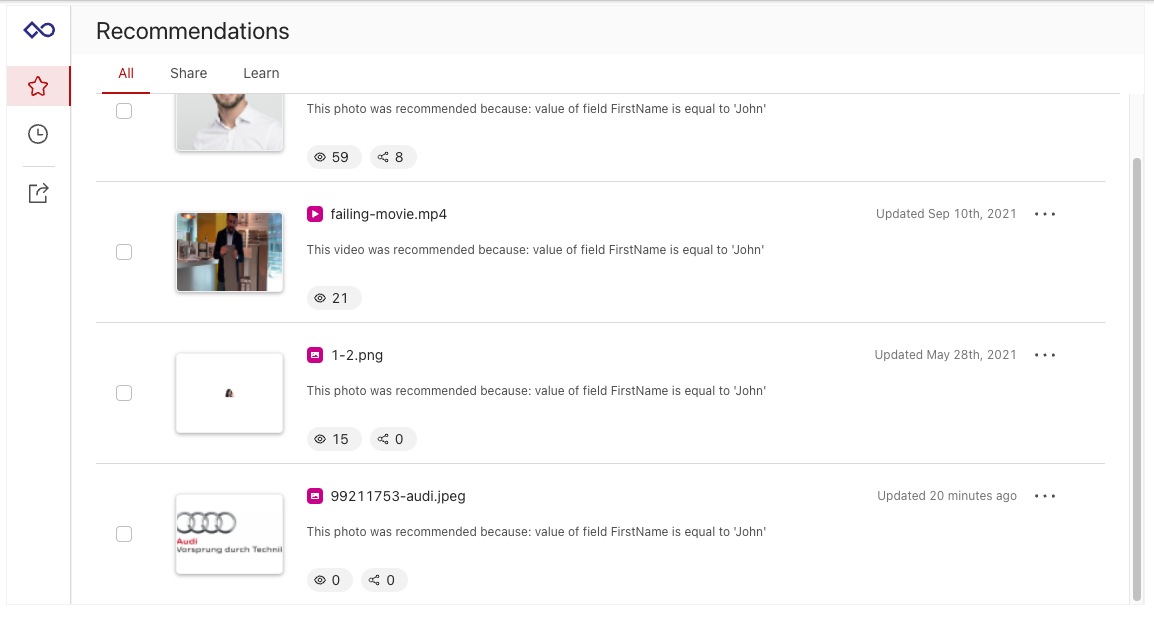
\includegraphics[width=12cm]{crm-widget}
    \caption{CRM widget}
\end{figure}

\section{Steps to Extract}
Decoupling the existing application
Setting up the environment
Running application on different port
Feature flag in central station to hide the mfe behind
Fixing stuff until it worked
\section{Challenges}
Following conventions and fitting it to our needs
Merging changes into master
Dependency issues, forgetting to import some dependencies
Setting it up for testers

The main challenge was because we are using a monorepo architecture and we’re trying to decouple parts/libraries from this highly dependent structure…
what does it mean in practice for our case:
dependencies -> for example asset viewer, external modules (npm modules), application state/store, authorisation
feature flag/routing -> deciding the convention to be used by the company for this purpose… either with different routes and guards or going against the best practices and hacking the route
keeping up with the metamorphosis of the monorepo… all the changes coming from master related or not with micro front ends
all of the unknown errors which we came to discover while running it… a major part was very vague from angular side.
